\section{Problem 3: Training on ImageNet from Scratch}
\label{sec:p3}

All models in this section are trained from random initialization; no pre-trained weights are used.
The code is in \texttt{problem3/} of our repository: \texttt{make\_prototype.py} builds the splits, \texttt{resnet\_custom.py} defines the ResNets and the activation, and \texttt{train\_imagenet.py} trains on one or several NVIDIA GPUs or Intel Gaudi cards with distributed data parallelism (DDP).

%-------------------------------------------------------------------------
\subsection{Train/validation/test splits and the prototype dataset}
\label{sec:p3-proto}

\paragraph{Full split.}
Only the ImageNet~\cite{deng2009imagenet} \emph{train} folder on Sol (\path{/data/datasets/community/deeplearning/imagenet/train}) has labels, so all our splits come from it.
The Sol copy contains 650 of the 1{,}000 ImageNet classes.
Within every class we shuffle the images (seed 0) and assign 80\% to training, 10\% to validation and 10\% to testing.
Every class therefore appears in every split, and the full test set has 83{,}257 images.
No image is copied: the split is a CSV manifest of paths and labels that the data loader reads, so the images stay in place on Sol.
\TODO{total number of images and the min/max images per class, from \texttt{proto\_summary.txt}.}

\paragraph{Prototype.}
The prototype has 100 classes with 300 images each, split 240/30/30, for 24{,}000 training, 3{,}000 validation and 3{,}000 test images.
The classes are spaced evenly through the sorted list of WordNet IDs.
Sorted IDs roughly group related concepts, so even spacing covers all super-categories (animals, objects, scenes) instead of, for example, 100 dog breeds.
The images are drawn from each split of the full dataset separately, so every prototype test image is also a full-dataset test image and the prototype never trains on full-dataset test images.
\Cref{fig:p3-proto-samples,fig:p3-proto-stats} summarize the prototype.
\TODO{image-size, aspect-ratio and color-mode statistics from \texttt{proto\_summary.txt}.}

\begin{figure*}[t]
  \centering
  \figorbox{\textwidth}{fig_proto_samples.png}{One example image of each of the first 40 prototype classes, with class names (made by \texttt{make\_prototype.py}).}
  \caption{Examples from the prototype dataset, one image per class.}
  \label{fig:p3-proto-samples}
\end{figure*}

\begin{figure*}[t]
  \centering
  \figorbox{\textwidth}{fig_proto_stats.png}{Class availability, split sizes, image sizes and aspect ratios (made by \texttt{make\_prototype.py}).}
  \caption{Statistics of the prototype dataset: images available per ImageNet class with the 100 prototype classes highlighted, split sizes, and the distribution of image sizes and aspect ratios.}
  \label{fig:p3-proto-stats}
\end{figure*}

%-------------------------------------------------------------------------
\subsection{A custom 36-layer ResNet}
\label{sec:p3-resnet36}

\paragraph{Design.}
ResNet-34~\cite{he2016resnet} has four stages of $[3,4,6,3]$ basic blocks (two $3\times3$ convolutions and a skip connection each).
Our ResNet-36 adds one basic block to the third stage, giving $[3,4,7,3]$ (\cref{tab:p3-arch}).
Counted like the original paper (convolutions and the fully connected layer on the main path, without the $1\times1$ projection shortcuts), that is $1+2\times17+1=36$ layers.
Following Goyal et al.~\cite{goyal2017accurate}, convolutions use Kaiming initialization and the last batch-norm scale $\gamma$ in every block starts at zero, so each residual block starts as an identity mapping.

\begin{table}[t]
  \centering
  \small
  \setlength{\tabcolsep}{4pt}
  \resizebox{\linewidth}{!}{%
  \begin{tabular}{@{}lccc@{}}
    \toprule
    Stage (output) & Block & ResNet-34 & ResNet-36 \\
    \midrule
    Stem ($56\times56$) & \makecell{$7\times7$, 64, stride 2\\$3\times3$ max-pool, stride 2} & 1 & 1 \\
    Stage 1 ($56\times56$) & $[3\times3, 64]\times2$ & $\times3$ & $\times3$ \\
    Stage 2 ($28\times28$) & $[3\times3, 128]\times2$ & $\times4$ & $\times4$ \\
    Stage 3 ($14\times14$) & $[3\times3, 256]\times2$ & $\times6$ & $\times\mathbf{7}$ \\
    Stage 4 ($7\times7$) & $[3\times3, 512]\times2$ & $\times3$ & $\times3$ \\
    Head ($1\times1$) & avg-pool, fully connected & 1 & 1 \\
    \midrule
    \multicolumn{2}{@{}l}{Weighted layers} & 34 & 36 \\
    \multicolumn{2}{@{}l}{Parameters (100 classes)} & 21.34\,M & 22.52\,M \\
    \multicolumn{2}{@{}l}{Parameters (650 classes)} & 21.62\,M & 22.80\,M \\
    \multicolumn{2}{@{}l}{Multiply-accumulates per image} & 3.66\,G & 3.90\,G \\
    \bottomrule
  \end{tabular}}
  \caption{ResNet-34 and our ResNet-36. The only difference is one extra basic block in the $14\times14$ stage.}
  \label{tab:p3-arch}
\end{table}

\paragraph{Expected benefit.}
We put the extra block in the $14\times14$ stage for three reasons.
\begin{enumerate}[nosep,leftmargin=*]
  \item This is the stage that deeper ResNets grow: ResNet-101 and ResNet-152 have 23 and 36 blocks there~\cite{he2016resnet}. At $14\times14$, the receptive fields cover object parts, so extra depth adds capacity to combine parts into objects, which is what separates fine-grained classes.
  \item It is cheap: the block adds 1.18\,M parameters (+5.5\%) and 0.23\,G multiply-accumulates (+6.3\%). A block in the last stage would add 4.7\,M parameters, and one in the first two stages would cost more computation at higher resolution.
  \item The skip connection and the zero-initialized $\gamma$ make the new block start as an identity mapping, so it does not disturb the signal early in training and is only used as far as it lowers the loss.
\end{enumerate}
We expect a small accuracy gain over ResNet-34, at most about 1 point, for a 6\% higher training cost.
On the small prototype the gain may be hidden by run-to-run noise or overfitting.

\paragraph{Training recipe (all prototype runs).}
SGD with Nesterov momentum 0.9 and a learning rate of 0.1 per 256 images, scaled linearly with the global batch~\cite{goyal2017accurate}.
Weight decay $5\cdot10^{-4}$, not applied to batch-norm parameters and biases.
Two warm-up epochs followed by a cosine decay~\cite{loshchilov2017sgdr}.
Label smoothing 0.1~\cite{szegedy2016inception}, batch size 128 per GPU, bfloat16 mixed precision.
Training augmentation is a random resized crop to $224\times224$ and a random horizontal flip; evaluation resizes to 256 and takes the $224\times224$ center crop.
We train for 30 epochs, keep the epoch with the best validation top-1 accuracy, and report its test accuracy.

\begin{table}[t]
  \centering
  \small
  \setlength{\tabcolsep}{4pt}
  \begin{tabular}{@{}lccccc@{}}
    \toprule
    Model & Params & \makecell{Val.\\top-1} & \makecell{Test\\top-1} & \makecell{Test\\top-5} & \makecell{Train\\time} \\
    \midrule
    ResNet-34 & 21.34\,M & \todo{--} & \todo{--} & \todo{--} & \todo{--} \\
    ResNet-36 (ours) & 22.52\,M & \todo{--} & \todo{--} & \todo{--} & \todo{--} \\
    \bottomrule
  \end{tabular}
  \caption{ResNet-34 vs.\ ResNet-36 on the prototype (100 classes, 30 epochs, ReLU). \TODO{copy \texttt{val\_top1}, \texttt{test\_top1}, \texttt{test\_top5} and \texttt{train\_time\_min} from \texttt{runs/resnet34/results.json} and \texttt{runs/resnet36/results.json}.}}
  \label{tab:p3-depth}
\end{table}

\begin{figure}[t]
  \centering
  \figorbox{\linewidth}{p3_depth_comparison.png}{Learning curves of ResNet-34 and ResNet-36 (\texttt{runs/comparison.png} from \texttt{compare\_runs.py}).}
  \caption{Training loss and validation accuracy of ResNet-34 and ResNet-36 on the prototype.}
  \label{fig:p3-depth}
\end{figure}

\paragraph{Result.}
\TODO{2--3 sentences on \cref{tab:p3-depth,fig:p3-depth}: did ResNet-36 beat ResNet-34, by how much, and at what extra training time?}

%-------------------------------------------------------------------------
\subsection{A custom activation function: ArcGate}
\label{sec:p3-arcgate}

\paragraph{Definition.}
Several modern activations gate the input by a cumulative distribution function (CDF): ReLU uses a hard step, SiLU/Swish~\cite{ramachandran2017swish} the logistic function, GELU~\cite{hendrycks2016gelu} the Gaussian CDF.
ArcGate gates with the CDF of the heavy-tailed Cauchy distribution:
\begin{align}
  f(x)  &= x\left(\frac12+\frac{\arctan x}{\pi}\right), \label{eq:arcgate}\\
  f'(x) &= \frac12+\frac{\arctan x}{\pi}+\frac{x}{\pi(1+x^2)}. \label{eq:arcgate-grad}
\end{align}
ArcGate is not available in PyTorch.
We implemented it as a custom \texttt{torch.autograd.Function} with the analytic derivative of \cref{eq:arcgate-grad}, which stores only the input for the backward pass (\cref{lst:p3-arcgate}).
It replaces every ReLU of the ResNet-36, including the one in the stem.

\begin{lstlisting}[caption={ArcGate with a hand-written backward pass (from \texttt{resnet\_custom.py}, lightly reformatted).},label={lst:p3-arcgate},float=t]
class _ArcGateFn(torch.autograd.Function):
    @staticmethod
    def forward(ctx, x):
        ctx.save_for_backward(x)
        return x * (0.5 + torch.atan(x) / math.pi)

    @staticmethod
    def backward(ctx, grad_out):
        (x,) = ctx.saved_tensors
        d = (0.5 + torch.atan(x) / math.pi
             + x / (math.pi * (1 + x * x)))  # f'(x)
        return grad_out * d
\end{lstlisting}

\begin{figure*}[t]
  \centering
  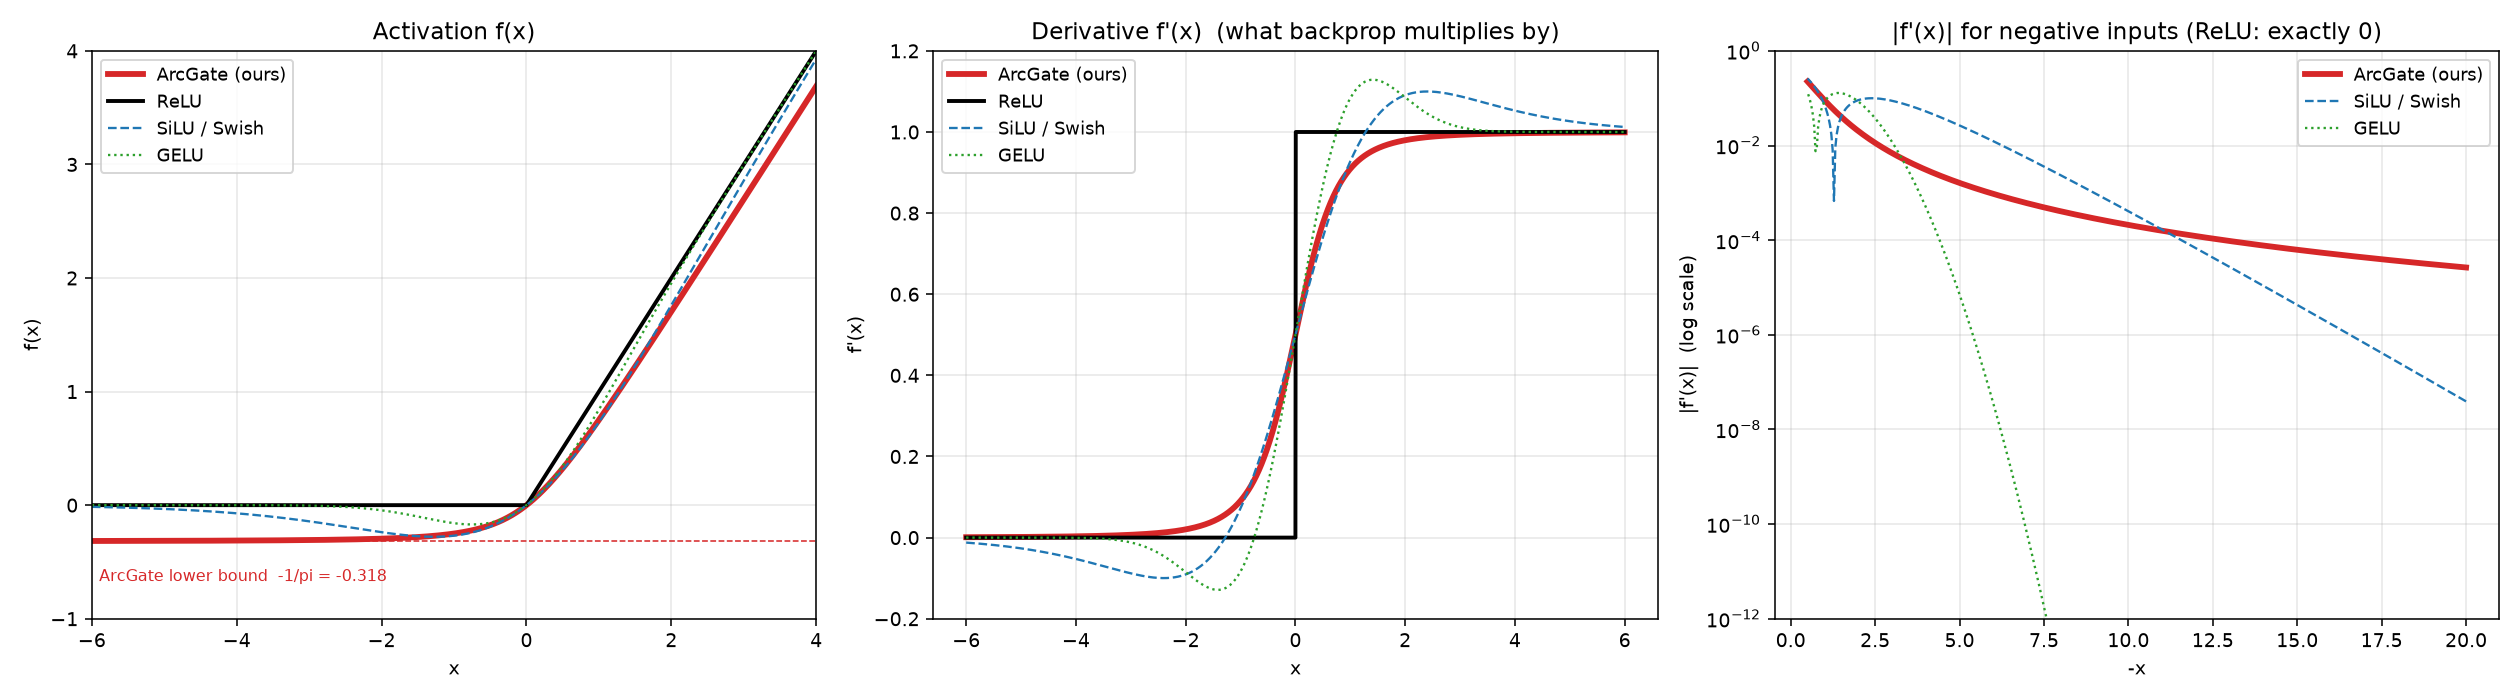
\includegraphics[width=\textwidth]{figs/p3_activation.png}
  \caption{ArcGate compared with ReLU, SiLU and GELU. Left: the activation $f(x)$; ArcGate is bounded below by $-1/\pi$. Middle: the derivative, which is what backpropagation multiplies by. Right: the derivative magnitude for negative inputs on a log scale; ArcGate's decays polynomially ($\propto|x|^{-3}$), SiLU's and GELU's exponentially, and ReLU's is exactly zero.}
  \label{fig:p3-activation}
\end{figure*}

\paragraph{Properties (\cref{fig:p3-activation}).}
\begin{itemize}[nosep,leftmargin=*]
  \item Smooth everywhere, with $f(0)=0$, $f'(0)=\tfrac12$, $f(1)=0.75$ and $f(-1)=-0.25$.
  \item \emph{Monotonic}: $f'(x)>0$ for all $x$ (checked numerically on $[-50,50]$). SiLU and GELU dip below zero and come back (minima $-0.28$ and $-0.17$); ArcGate keeps decreasing towards its lower bound $-1/\pi\approx-0.318$.
  \item For large positive inputs $f(x)\approx x-1/\pi$, so it behaves like a shifted identity.
  \item For large negative inputs the gradient decays only polynomially, $f'(x)\approx 2/(3\pi|x|^3)$, compared with exponentially for SiLU and GELU and exactly zero for ReLU.
\end{itemize}

\paragraph{Expectations.}
Like other smooth gated activations, ArcGate should give a smoother loss surface and slightly better optimization than ReLU.
Because its gradient is never exactly zero, no unit can ``die''.
Its small negative outputs pull the mean activation towards zero, which can help optimization.
On the cost side, $\arctan$ is more expensive than $\max(0,x)$, and the custom backward cannot be fused like ReLU's, so we expect each epoch to be somewhat slower.
The heavy tail also makes the activations less sparse than with ReLU.

\begin{table}[t]
  \centering
  \small
  \setlength{\tabcolsep}{4pt}
  \begin{tabular}{@{}lcccc@{}}
    \toprule
    ResNet-36 with & \makecell{Val.\\top-1} & \makecell{Test\\top-1} & \makecell{Test\\top-5} & \makecell{Time per\\epoch} \\
    \midrule
    ReLU & \todo{--} & \todo{--} & \todo{--} & \todo{--} \\
    ArcGate (ours) & \todo{--} & \todo{--} & \todo{--} & \todo{--} \\
    \bottomrule
  \end{tabular}
  \caption{ReLU vs.\ ArcGate in ResNet-36 on the prototype (30 epochs, everything else identical). \TODO{copy from \texttt{runs/resnet36/results.json} and \texttt{runs/resnet36\_arcgate/results.json}; time per epoch = \texttt{train\_time\_min} / \texttt{epochs}.}}
  \label{tab:p3-act}
\end{table}

\begin{figure}[t]
  \centering
  \figorbox{\linewidth}{p3_activation_comparison.png}{Learning curves of ResNet-36 with ReLU and with ArcGate (\texttt{runs/activation\_comparison.png}).}
  \caption{Training loss and validation accuracy of ResNet-36 with ReLU and with ArcGate on the prototype.}
  \label{fig:p3-act}
\end{figure}

\paragraph{Result.}
\TODO{2--3 sentences on \cref{tab:p3-act,fig:p3-act}: compare accuracy and speed and say whether the expectations above held.}

%-------------------------------------------------------------------------
\subsection{Training on the full dataset}
\label{sec:p3-full}

We trained ResNet-36 with ArcGate on the full 650-class split for 10 epochs with the hyperparameters of \cref{tab:p3-full-hparams}, and evaluated the best-validation epoch on the 83{,}257 test images (\cref{tab:p3-full-results}).

\begin{table}[t]
  \centering
  \small
  \begin{tabular}{@{}ll@{}}
    \toprule
    Setting & Value \\
    \midrule
    Model & ResNet-36 + ArcGate, 22.80\,M parameters \\
    Data & full split: 650 classes, 80/10/10 \\
    Hardware & \TODO{device(s) used for this run} \\
    Epochs & 10 \\
    Global batch & 256 (2 devices $\times$ 128, DDP) \\
    Optimizer & SGD, Nesterov momentum 0.9 \\
    Learning rate & 0.1, 1 warm-up epoch, cosine decay \\
    Weight decay & $10^{-4}$ (none on norms and biases) \\
    Label smoothing & 0.1 \\
    Precision & bfloat16 mixed precision \\
    Augmentation & random resized crop 224, horizontal flip \\
    \bottomrule
  \end{tabular}
  \caption{Hyperparameters of the full-dataset run.}
  \label{tab:p3-full-hparams}
\end{table}

\begin{table}[t]
  \centering
  \small
  \begin{tabular}{@{}lcc@{}}
    \toprule
    \multicolumn{3}{@{}l}{\textbf{Accuracy}} \\
    Split & Top-1 & Top-5 \\
    \midrule
    Train (augmented, best epoch) & 54.4\% & -- \\
    Validation & 60.0\% & 82.6\% \\
    Test (83{,}257 images) & \textbf{60.4\%} & \textbf{82.9\%} \\
    \midrule
    \multicolumn{3}{@{}l}{\textbf{Time and latency}} \\
    \midrule
    \multicolumn{2}{@{}l}{Training time (10 epochs, training only)} & 53.9 min \\
    \multicolumn{2}{@{}l}{\quad per epoch (epoch 1, incl.\ cold start)} & 5.4 (8.3) min \\
    \multicolumn{2}{@{}l}{Total job time (with validation, test, latency)} & 63.1 min \\
    \multicolumn{2}{@{}l}{Training throughput} & 2{,}120 img/s \\
    \multicolumn{2}{@{}l}{Test-set evaluation (83{,}257 images)} & 80 s \\
    \multicolumn{2}{@{}l}{Inference latency, batch 1 (median / p90)} & 6.19 / 6.28 ms \\
    \multicolumn{2}{@{}l}{\quad throughput at batch 1} & 161 img/s \\
    \multicolumn{2}{@{}l}{Inference, batch 64 (per batch)} & 7.7 ms \\
    \multicolumn{2}{@{}l}{\quad throughput at batch 64} & 8{,}286 img/s \\
    \bottomrule
  \end{tabular}
  \caption{ResNet-36 + ArcGate on the full dataset: accuracy, training time and inference latency (bfloat16, data loading excluded from latency).}
  \label{tab:p3-full-results}
\end{table}

\paragraph{Discussion.}
\begin{itemize}[nosep,leftmargin=*]
  \item \emph{No overfitting.} The training accuracy (54.4\%) is below the validation accuracy (60.0\%). It is measured on random resized crops with label smoothing, which are much harder than the center crops used for evaluation. Validation and test accuracy agree within 0.4 points, so the validation set is a reliable model-selection signal.
  \item \emph{The model is under-trained.} Ten epochs are far fewer than the usual 90. For reference, the torchvision ResNet-34 reaches 73.3\% top-1 on the 1{,}000-class ImageNet after 90 epochs; that number is not directly comparable (different classes and test set), but it shows how much longer training would add.
  \item \emph{Speed.} One epoch takes 5.4 minutes at $\approx$2{,}120 images/s; the first epoch is slower (8.3 minutes) because of start-up costs. The whole run takes about an hour.
  \item \emph{Latency.} A single image takes 6.2\,ms, but a batch of 64 takes only 7.7\,ms, i.e., 51 times the throughput. At batch size 1 the accelerator is mostly idle and the time is dominated by fixed per-layer overheads, so batching is essential for deployment throughput.
\end{itemize}

%-------------------------------------------------------------------------
\subsection{Vision Transformer comparison}
\label{sec:p3-vit}

\paragraph{Model and recipe.}
We chose ViT-S/16~\cite{dosovitskiy2021vit,touvron2021deit}: 12 transformer blocks, 384-dimensional tokens, 6 attention heads, MLP size 1{,}536 and $16\times16$ patches, built with torchvision's \texttt{VisionTransformer} and initialized randomly.
With 650 classes it has 21.92\,M parameters, almost the same as ResNet-36 (22.80\,M), which makes the comparison fair.
It uses the same split, epochs, global batch, augmentation, label smoothing and precision as the ResNet.
The optimizer follows the DeiT recipe~\cite{touvron2021deit} for transformers: AdamW with a learning rate of $5\cdot10^{-4}$ per 512 images, weight decay 0.05 (none on norms, biases, the class token and the position embeddings), gradient-norm clipping at 1.0, one warm-up epoch and cosine decay.

\paragraph{Expectation.}
A ViT has no built-in locality or translation equivariance; it must learn these from data.
DeiT needs 300 epochs and strong augmentation to match CNNs on ImageNet~\cite{touvron2021deit}.
With only 10 epochs and light augmentation we therefore expect ResNet-36 to clearly outperform the ViT.

\begin{table*}[t]
  \centering
  \small
  \setlength{\tabcolsep}{8pt}
  \begin{tabular}{@{}lcccccc@{}}
    \toprule
    Model & Params & \makecell{Test\\top-1} & \makecell{Test\\top-5} & \makecell{Train\\time} & \makecell{Latency\\b=1} & \makecell{Throughput\\b=64} \\
    \midrule
    ResNet-36 + ArcGate & 22.80\,M & 60.4\% & 82.9\% & 53.9 min & 6.2 ms & 8{,}286/s \\
    ViT-S/16 & 21.92\,M & \todo{--} & \todo{--} & \todo{--} & \todo{--} & \todo{--} \\
    \bottomrule
  \end{tabular}
  \caption{Custom ResNet-36 with ArcGate vs.\ ViT-S/16, both trained from scratch on the full 650-class split for 10 epochs. \TODO{copy the ViT numbers from \texttt{runs\_full/vit\_s16\_gpu/results.json}.}}
  \label{tab:p3-vit}
\end{table*}

\paragraph{Result.}
\TODO{2--3 sentences on \cref{tab:p3-vit}: does the ViT outperform the custom ResNet? Explain with the expectation above.}
